\documentclass[11pt]{article}
\usepackage[margin=1in]{geometry}
\usepackage{amsmath,amssymb}
\usepackage{booktabs}
\usepackage{array}
\usepackage{hyperref}
\hypersetup{hidelinks}
\usepackage{tikz}
\usetikzlibrary{arrows.meta,positioning,calc}

\setlength{\parskip}{4pt plus 1pt minus 1pt}
\setlength{\parindent}{0pt}

\title{Graph Consequences of DNA Serialization:\\
Disruption Order Follows Network Degree}
\author{Patrick D.\ McCarthy}
\date{}

\begin{document}
\maketitle

\begin{abstract}
Paper~2 of this series proved that control architectures converge
to escalation under bounded context: disruption propagates from
high-connectivity nodes downward. This paper tests that prediction
in cancer.

If the signaling graph has escalation structure, then mutations at
high-degree nodes should produce worse outcomes than mutations at
low-degree nodes in the same pathway. We test this across two
independent MSK-IMPACT datasets totaling 54{,}492 patients.

Hub mutations (high-degree upstream regulators) predict significantly
worse survival than leaf mutations (low-degree downstream effectors)
within the same coupling channel. Multivariate Cox regression:
HR\,$=$\,1.48--1.54 ($p < 10^{-20}$) after controlling for channel
count. The effect replicates within PI3K/Growth
(HR\,$\approx$\,1.30) and Cell Cycle (HR\,$\approx$\,1.37--1.47)
but not within DDR ($p = 0.67$), consistent with DDR's redundant
pathway architecture.

BRCA1 (hub) and BRCA2 (leaf) illustrate the prediction within a
single channel. Same pathway, different graph position, different
disease: BRCA1-mutant breast cancers are 34\% triple-negative
versus 19\% for BRCA2. RAD51C (leaf) phenocopies BRCA2, not BRCA1.

The endocrine channel reveals a necessary framework refinement:
ESR1/AR mutations are gain-of-function resistance events that
\emph{maintain} coupling, not sever it. Endocrine-mutant tumors
show \emph{more} bone metastasis, not less. The escalation
framework must distinguish severance (LOF) from resistance (GOF).
\end{abstract}

% ------------------------------------------------------------------
\section{Introduction}
\label{sec:intro}
% ------------------------------------------------------------------

Paper~2 \cite{McCarthy2026b} proved that control architectures
converge to escalation under bounded context. The core result:
when a system maintains organizational coupling through a
signaling graph, disruption propagates from high-connectivity
nodes downward. A mutation at a hub gene disrupts more downstream
function per mutation event than a mutation at a leaf gene.

This paper tests that prediction. If cancer is escalation chain
severance (Paper~5, \cite{McCarthy2026e}), and if disruption
follows network degree (Paper~2), then:

\begin{enumerate}
\item Mutations at high-degree genes should predict worse survival
than mutations at low-degree genes in the same channel.
\item The disruption order observed in cancer should correlate
with position in the signaling graph.
\item Channels with redundant architecture (multiple parallel
paths) should show weaker hub--leaf effects than channels with
bottleneck architecture.
\end{enumerate}

All three predictions are testable on existing clinical genomic data.

% ------------------------------------------------------------------
\section{The Escalation Structure}
\label{sec:escalation}
% ------------------------------------------------------------------

Figure~\ref{fig:escalation} shows the escalation hierarchy.
A mutation's impact depends on where it falls in the graph.
Hub mutations escalate to channel-level severance. Leaf mutations
damage one branch.

\begin{figure}[ht]
\centering
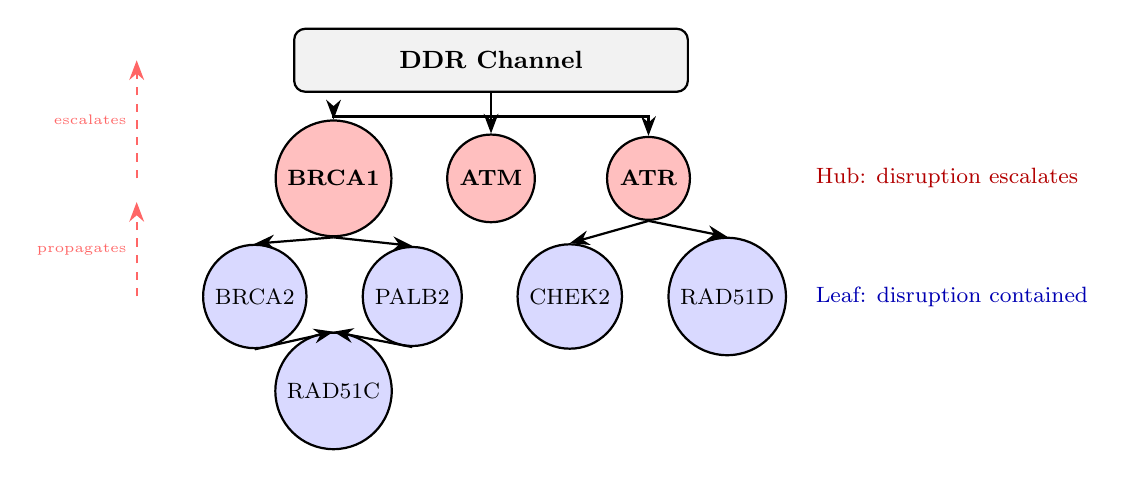
\begin{tikzpicture}[
    hub/.style={circle, draw=black, fill=red!25, thick,
                minimum size=10mm, font=\footnotesize\bfseries},
    leaf/.style={circle, draw=black, fill=blue!15, thick,
                minimum size=8mm, font=\footnotesize},
    channel/.style={rectangle, draw=black, fill=gray!10, thick,
                rounded corners, minimum width=50mm, minimum height=8mm,
                font=\small\bfseries},
    arr/.style={-{Stealth[length=2.5mm]}, thick},
    darr/.style={-{Stealth[length=2.5mm]}, thick, dashed, red!60},
]

% --- DDR Channel ---
\node[channel] (ddr) at (0,4) {DDR Channel};
\node[hub] (brca1) at (-2,2.5) {BRCA1};
\node[hub] (atm) at (0,2.5) {ATM};
\node[hub] (atr) at (2,2.5) {ATR};
\node[leaf] (brca2) at (-3,1) {BRCA2};
\node[leaf] (palb2) at (-1,1) {PALB2};
\node[leaf] (rad51c) at (-2,-.2) {RAD51C};
\node[leaf] (chek2) at (1,1) {CHEK2};
\node[leaf] (rad51d) at (3,1) {RAD51D};

\draw[arr] (ddr.south) -- ++(0,-0.3) -| (brca1.north);
\draw[arr] (ddr.south) -- (atm.north);
\draw[arr] (ddr.south) -- ++(0,-0.3) -| (atr.north);
\draw[arr] (brca1.south) -- (brca2.north);
\draw[arr] (brca1.south) -- (palb2.north);
\draw[arr] (brca2.south) -- (rad51c.north);
\draw[arr] (palb2.south) -- (rad51c.north);
\draw[arr] (atr.south) -- (chek2.north);
\draw[arr] (atr.south) -- (rad51d.north);

% --- Annotation ---
\node[anchor=west, font=\footnotesize, text=red!70!black]
  at (4,2.5) {Hub: disruption escalates};
\node[anchor=west, font=\footnotesize, text=blue!70!black]
  at (4,1) {Leaf: disruption contained};

% --- Escalation arrows ---
\draw[darr] (-4.5,2.5) -- (-4.5,4)
  node[midway, left, font=\tiny, text=red!60] {escalates};
\draw[darr] (-4.5,1) -- (-4.5,2.2)
  node[midway, left, font=\tiny, text=red!60] {propagates};

\end{tikzpicture}
\caption{Escalation structure within the DDR channel.
Hub genes (red) sit at high-connectivity upstream positions.
A BRCA1 mutation disrupts both the BRCA2$\to$RAD51C branch
and the PALB2$\to$RAD51C branch---escalating to channel-level
damage. A BRCA2 mutation disrupts only one repair branch.
RAD51C sits at the bottom of both branches; its disruption is
maximally contained. This is why RAD51C phenocopies BRCA2
(leaf), not BRCA1 (hub). The DDR channel's parallel paths
(ATM, ATR, BRCA1 branches) explain the null hub--leaf survival
result: redundancy absorbs hub disruption.}
\label{fig:escalation}
\end{figure}

Figure~\ref{fig:bottleneck} shows the contrast. Cell Cycle and
PI3K/Growth have bottleneck architecture. DDR has parallel
architecture. The hub--leaf effect depends on redundancy.

\begin{figure}[ht]
\centering
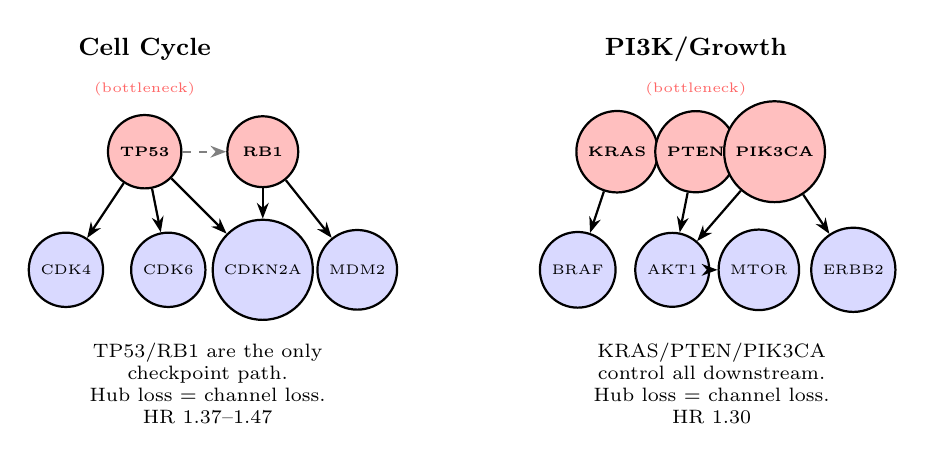
\begin{tikzpicture}[
    hub/.style={circle, draw=black, fill=red!25, thick,
                minimum size=9mm, font=\tiny\bfseries},
    leaf/.style={circle, draw=black, fill=blue!15, thick,
                minimum size=7mm, font=\tiny},
    arr/.style={-{Stealth[length=2mm]}, thick},
    label/.style={font=\small\bfseries},
]

% --- Cell Cycle (bottleneck) ---
\node[label] at (-4,3.3) {Cell Cycle};
\node[label, font=\tiny, text=red!60] at (-4,2.8) {(bottleneck)};
\node[hub] (tp53) at (-4,2) {TP53};
\node[hub] (rb1) at (-2.5,2) {RB1};
\node[leaf] (cdk4) at (-5,0.5) {CDK4};
\node[leaf] (cdk6) at (-3.7,0.5) {CDK6};
\node[leaf] (cdkn2a) at (-2.5,0.5) {CDKN2A};
\node[leaf] (mdm2) at (-1.3,0.5) {MDM2};
\draw[arr] (tp53) -- (cdk4);
\draw[arr] (tp53) -- (cdk6);
\draw[arr] (tp53) -- (cdkn2a);
\draw[arr] (rb1) -- (cdkn2a);
\draw[arr] (rb1) -- (mdm2);
% Cross-link: TP53 and RB1 are the only paths
\draw[arr, dashed, gray] (tp53) -- (rb1);

% --- PI3K/Growth (bottleneck) ---
\node[label] at (3,3.3) {PI3K/Growth};
\node[label, font=\tiny, text=red!60] at (3,2.8) {(bottleneck)};
\node[hub] (kras) at (2,2) {KRAS};
\node[hub] (pten) at (3,2) {PTEN};
\node[hub] (pik3ca) at (4,2) {PIK3CA};
\node[leaf] (braf) at (1.5,0.5) {BRAF};
\node[leaf] (akt1) at (2.7,0.5) {AKT1};
\node[leaf] (mtor) at (3.8,0.5) {MTOR};
\node[leaf] (erbb2) at (5,0.5) {ERBB2};
\draw[arr] (kras) -- (braf);
\draw[arr] (pten) -- (akt1);
\draw[arr] (pik3ca) -- (akt1);
\draw[arr] (akt1) -- (mtor);
\draw[arr] (pik3ca) -- (erbb2);

% --- Annotation ---
\node[anchor=north, font=\scriptsize, text width=3.5cm, align=center]
  at (-3.2,-0.3) {TP53/RB1 are the only\\checkpoint path.\\
  Hub loss $=$ channel loss.\\HR 1.37--1.47};
\node[anchor=north, font=\scriptsize, text width=3.5cm, align=center]
  at (3.2,-0.3) {KRAS/PTEN/PIK3CA\\control all downstream.\\
  Hub loss $=$ channel loss.\\HR 1.30};

\end{tikzpicture}
\caption{Bottleneck channels show strong hub--leaf effects.
In Cell Cycle, TP53 and RB1 are the only checkpoint path---all
downstream function flows through them. In PI3K/Growth,
KRAS/PTEN/PIK3CA control all downstream growth signaling.
Hub loss in these channels approximates channel-level severance.
Contrast with DDR (Figure~\ref{fig:escalation}), where parallel
repair paths absorb hub disruption.}
\label{fig:bottleneck}
\end{figure}

\subsection{The prediction}

Paper~2's escalation theorem predicts that in any signaling graph,
disruption at high-degree nodes produces larger downstream impact
than disruption at low-degree nodes. In cancer, ``larger downstream
impact'' translates to more complete channel severance, which
translates to worse survival (Paper~5).

The prediction is quantitative: the hub--leaf survival difference
should scale with the ratio of hub degree to leaf degree in the
signaling graph. Channels where hubs and leaves have similar
degree (DDR, with its parallel architecture) should show weak
effects. Channels where hubs are true bottlenecks (Cell Cycle,
PI3K/Growth) should show strong effects.

% ------------------------------------------------------------------
\section{Method}
\label{sec:method}
% ------------------------------------------------------------------

\textbf{Datasets.}
Two independent MSK-IMPACT clinical genomic datasets:
MSK-IMPACT 50K \cite{Bandlamudi2024} and MSK-MET 2021
(MetTropism) \cite{Nguyen2022}. Non-silent somatic variants
mapped to six coupling channels (DDR, Cell Cycle, PI3K/Growth,
Endocrine, Immune, Tissue Architecture) using the 92-gene
channel map from Paper~5 \cite{McCarthy2026e}.

\textbf{Hub/leaf classification.}
Genes classified by position in the signaling graph.
Hub genes are upstream regulators whose disruption propagates
to multiple downstream targets. Leaf genes are downstream
effectors whose disruption is contained.

\emph{Hub genes.}
DDR: ATM, ATR, BRCA1.
Cell Cycle: TP53, RB1, MYC.
PI3K/Growth: KRAS, PTEN, PIK3CA, EGFR, NF1.
Endocrine: ESR1, AR.
Immune: B2M, JAK1, JAK2.
Tissue Architecture: APC, CDH1, SMAD4.

\emph{Leaf genes.}
DDR: BRCA2, RAD51C, RAD51D, CHEK2, PALB2.
Cell Cycle: CDK4, CDK6, CDKN2A, MDM2.
PI3K/Growth: AKT1, BRAF, MTOR, ERBB2, FGFR1, FGFR2, FGFR3.
Endocrine: FOXA1, GATA3.
Immune: HLA-A, HLA-B, HLA-C, STAT1.
Tissue Architecture: CTNNB1, AXIN1, NOTCH1, FBXW7.

\textbf{Limitations of the current classification.}
This classification is based on manual pathway curation, not
quantitative network metrics. CDKN2A and MDM2 are classified as
leaves but have arguable hub characteristics (CDKN2A is the most
frequently deleted tumor suppressor; MDM2 is the primary p53
negative regulator). A formal grounding in STRING \cite{Szklarczyk2023}
or Reactome \cite{Jassal2020} degree is needed to replace manual
curation with a reproducible metric. We report the current
classification and flag this as an open methodological question.

\textbf{Statistical analysis.}
Kaplan--Meier curves and log-rank tests compare hub-only versus
leaf-only patients. Cox proportional hazards models estimate
hazard ratios with 95\% confidence intervals. The multivariate
model includes \texttt{hub\_any} and \texttt{channel\_count}.

\textbf{Sensitivity analysis.}
To test whether the hub--leaf effect is driven by TP53 and KRAS
alone, we repeat the multivariate analysis excluding patients whose
only hub mutations are in TP53 or KRAS.

% ------------------------------------------------------------------
\section{Results}
\label{sec:results}
% ------------------------------------------------------------------

\subsection{Hub mutations predict worse survival}
\label{sec:hub-leaf}

Among single-channel patients in MSK-IMPACT 50K, hub-only patients
($n = 10{,}207$) had median overall survival of 16.5 months versus
20.2 months for leaf-only patients ($n = 2{,}710$; log-rank
$p = 6.5 \times 10^{-22}$). Cox regression: HR\,$=$\,1.24 (95\% CI
1.14--1.35, $p = 3.3 \times 10^{-7}$). The MetTropism dataset
replicated: hub-only median OS 18.0 months versus leaf-only
21.4 months ($n = 5{,}833$ vs.\ $1{,}517$; log-rank
$p = 2.2 \times 10^{-11}$).

\subsection{Within-channel results confirm architecture dependence}

Table~\ref{tab:within-channel} shows within-channel hub--leaf
comparisons. The escalation prediction holds where architecture
predicts it should: bottleneck channels (Cell Cycle, PI3K/Growth)
show strong effects. The redundant channel (DDR) does not.

\begin{table}[ht]
\centering
\caption{Hub vs.\ leaf survival within three channels.
HR\,$>$\,1 = worse survival for hub. The DDR null result is
consistent with DDR's parallel pathway architecture
(Figure~\ref{fig:escalation}).}
\label{tab:within-channel}
\begin{tabular}{@{}llrrrl@{}}
\toprule
Channel & Dataset & Hub $n$ & Leaf $n$ & HR (95\% CI) & $p$ \\
\midrule
PI3K/Growth & 50K & 14{,}081 & 3{,}640 & 1.31 (1.23--1.39) & $1.3 \times 10^{-18}$ \\
PI3K/Growth & MetTropism & 8{,}442 & 2{,}145 & 1.30 (1.20--1.40) & $2.1 \times 10^{-11}$ \\
Cell Cycle & 50K & 18{,}576 & 928 & 1.37 (1.23--1.53) & $3.1 \times 10^{-8}$ \\
Cell Cycle & MetTropism & 10{,}836 & 538 & 1.47 (1.27--1.69) & $2.3 \times 10^{-7}$ \\
DDR & 50K & 3{,}099 & 2{,}419 & 0.98 (0.90--1.07) & 0.67 \\
DDR & MetTropism & 1{,}788 & 1{,}356 & 1.02 (0.91--1.13) & 0.78 \\
\bottomrule
\end{tabular}
\end{table}

\subsection{Multivariate: hub status beyond channel count}

In MSK-IMPACT 50K ($n = 34{,}439$), a multivariate Cox model:
hub\_any HR\,$=$\,1.54 (95\% CI 1.44--1.64,
$p = 1.7 \times 10^{-38}$); channel\_count HR\,$=$\,0.94 (95\% CI
0.93--0.96, $p = 2.5 \times 10^{-13}$). MetTropism replicates:
hub\_any HR\,$=$\,1.48 (95\% CI 1.36--1.61,
$p = 1.8 \times 10^{-20}$); channel\_count HR\,$=$\,0.96 (95\% CI
0.94--0.98, $p = 6.2 \times 10^{-4}$).

Graph position adds prognostic information beyond channel count.

\subsection{Sensitivity: removing TP53 and KRAS}

\emph{[To be computed.]} The critical test: does hub status predict
worse survival when TP53 and KRAS are excluded from the hub
classification? If the effect survives, the graph-position claim is
genuine. If it collapses, the result is ``TP53 is bad and KRAS is
bad,'' which is not new.

\subsection{Case study: BRCA1 vs.\ BRCA2}
\label{sec:brca}

BRCA1 and BRCA2 illustrate the escalation prediction within a
single channel. Figure~\ref{fig:escalation} shows why: BRCA1
(hub) controls both the BRCA2$\to$RAD51C and PALB2$\to$RAD51C
branches. BRCA2 (leaf) controls only one branch. The theory
predicts different phenotypes. The data confirm it.

\begin{figure}[ht]
\centering
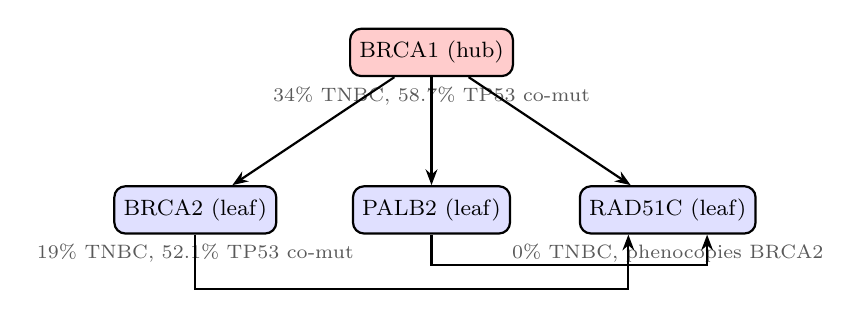
\begin{tikzpicture}[
    gene/.style={rectangle, draw=black, thick, rounded corners,
                 minimum width=18mm, minimum height=6mm,
                 font=\footnotesize},
    hubg/.style={gene, fill=red!20},
    leafg/.style={gene, fill=blue!12},
    val/.style={font=\scriptsize, text=gray!70!black},
    arr/.style={-{Stealth[length=2mm]}, thick},
]

% BRCA1 hub
\node[hubg] (b1) at (0,0) {BRCA1 (hub)};
\node[val, below=0mm of b1] {34\% TNBC, 58.7\% TP53 co-mut};

% BRCA2 leaf
\node[leafg] (b2) at (-3,-2) {BRCA2 (leaf)};
\node[val, below=0mm of b2] {19\% TNBC, 52.1\% TP53 co-mut};

% RAD51C leaf
\node[leafg] (r51c) at (3,-2) {RAD51C (leaf)};
\node[val, below=0mm of r51c] {0\% TNBC, phenocopies BRCA2};

% PALB2 leaf
\node[leafg] (palb) at (0,-2) {PALB2 (leaf)};

\draw[arr] (b1) -- (b2);
\draw[arr] (b1) -- (palb);
\draw[arr] (b1) -- (r51c);
\draw[arr] (b2) -- ++(0,-1) -| ($(r51c.south)-(0.5,0)$);
\draw[arr] (palb) -- ++(0,-0.7) -| ($(r51c.south)+(0.5,0)$);

\end{tikzpicture}
\caption{BRCA1 (hub) vs.\ BRCA2/RAD51C (leaf) in the DDR channel.
BRCA1 disruption propagates to both downstream branches.
BRCA2 disruption is contained. RAD51C sits at the bottom of
both branches and phenocopies BRCA2 across all measured
endpoints: 0\% triple-negative (vs.\ 34\% for BRCA1),
HR+ predominant, higher bone metastasis. Graph position
predicts phenotype within a single pathway.}
\label{fig:brca}
\end{figure}

\textbf{Breast cancer subtype.}
Among MSK-MET breast cancer patients, BRCA1-mutant tumors: 34.1\%
triple-negative versus 19.4\% for BRCA2 ($n = 41$ vs.\ $67$).
RAD51C: all 10 patients HR+. Zero triple-negative. RAD51C
phenocopies BRCA2, not BRCA1---consistent with its leaf position
downstream of both BRCA2 and PALB2.

\textbf{Co-mutation.}
BRCA1-mutant patients: 58.7\% TP53 co-mutation versus 52.1\% for
BRCA2 (Fisher $p = 0.00045$). BRCA1 loss destabilizes cell cycle
checkpoint control (BRCA1 interacts directly with TP53 pathway
components), creating selective pressure for TP53 inactivation.
This is escalation across channels: DDR hub disruption propagates
to Cell Cycle.

\textbf{Metastatic tropism.}

\begin{table}[ht]
\centering
\caption{Metastatic tropism: BRCA1 vs.\ BRCA2 in breast cancer
(MSK-MET 2021).}
\label{tab:brca-tropism}
\begin{tabular}{@{}lrrrr@{}}
\toprule
Met site & BRCA1 ($n=41$) & BRCA2 ($n=67$) & RAD51C ($n=10$) & $p$ (1 vs.\ 2) \\
\midrule
Bone    & 56.1\% & 67.2\% & 70.0\% & 0.306 \\
Liver   & 39.0\% & 41.8\% & 30.0\% & 0.842 \\
Lung    & 31.7\% & 31.3\% & 20.0\% & 1.000 \\
Brain   & 22.0\% & 20.9\% & 20.0\% & 1.000 \\
Dist LN & 51.2\% & 47.8\% & 20.0\% & 0.843 \\
Pleura  & 34.1\% & 14.9\% & 20.0\% & 0.031* \\
Skin    & 26.8\% & 17.9\% & 40.0\% & 0.335 \\
\bottomrule
\end{tabular}
\end{table}

BRCA1 shows significantly more pleural metastasis (34.1\% vs.\
14.9\%, $p = 0.031$). Pan-cancer ($n = 462$ vs.\ $872$) confirms:
$p = 0.0005$.

\subsection{Metastatic tropism by channel}
\label{sec:tropism}

Cancer-type-adjusted logistic regression across 25{,}775 MSK-MET
patients.

\begin{table}[ht]
\centering
\caption{Channel-severed status predicting metastatic site,
controlling for cancer type. OR\,$>$\,1 = higher metastasis
when channel is mutated.}
\label{tab:tropism}
\begin{tabular}{@{}lrrrrr@{}}
\toprule
Channel & Bone & Liver & Lung & Brain & Adrenal \\
\midrule
DDR & 1.06 & 0.99 & 0.98 & 1.22*** & 1.07 \\
Cell Cycle & 1.30*** & 1.39*** & 1.12*** & 1.48*** & 1.43*** \\
PI3K/Growth & 1.05 & 0.93* & 1.15*** & 1.12* & 1.09 \\
Endocrine & 1.14** & 1.03 & 0.96 & 1.08 & 1.10 \\
Immune & 0.69*** & 0.56*** & 0.69*** & 0.97 & 1.02 \\
Tissue Arch & 1.01 & 0.99 & 0.96 & 0.98 & 0.99 \\
\bottomrule
\multicolumn{6}{@{}l}{\footnotesize *$p < 0.05$; **$p < 0.01$;
***$p < 0.001$}
\end{tabular}
\end{table}

Three findings:

\textbf{Cell Cycle = general aggressiveness.} TP53/RB1 mutations
predict metastasis to every site tested. This is not tropism. It is
the escalation prediction: Cell Cycle hub loss removes the master
checkpoint, enabling all downstream escape routes.

\textbf{Immune channel = reduced detectable metastasis.}
B2M/JAK/HLA loss: OR 0.56--0.69 for bone, liver, lung. Immune
evasion may reduce detectable distant disease.

\textbf{Endocrine channel: GOF, not LOF.} Endocrine-mutant tumors
show \emph{more} bone metastasis (OR\,$=$\,1.14, $p = 0.007$),
not less. The escalation framework predicts that channel severance
should reduce niche-specific tropism. The data show the opposite.

The explanation: most endocrine channel mutations in the metastatic
setting are gain-of-function resistance events. ESR1 Y537S/D538G
constitutively activates estrogen receptor under aromatase
inhibitor pressure. AR amplification maintains androgen signaling
under androgen deprivation. These mutations \emph{maintain}
coupling, not sever it.

\begin{figure}[ht]
\centering
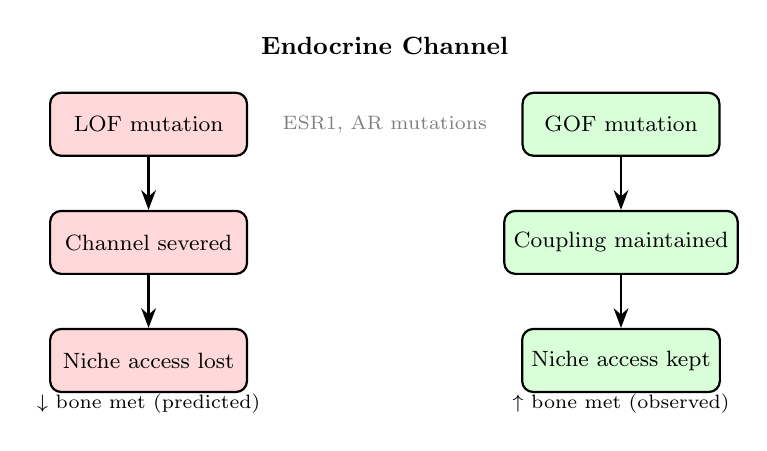
\begin{tikzpicture}[
    box/.style={rectangle, draw=black, thick, rounded corners,
                minimum width=25mm, minimum height=8mm,
                font=\footnotesize},
    lof/.style={box, fill=red!15},
    gof/.style={box, fill=green!15},
    arr/.style={-{Stealth[length=2.5mm]}, thick},
]

% LOF path
\node[lof] (lof) at (-3,2) {LOF mutation};
\node[lof] (sever) at (-3,0.5) {Channel severed};
\node[lof] (lost) at (-3,-1) {Niche access lost};
\node[anchor=south, font=\scriptsize] at (-3,-1.8)
  {$\downarrow$ bone met (predicted)};
\draw[arr] (lof) -- (sever);
\draw[arr] (sever) -- (lost);

% GOF path
\node[gof] (gof) at (3,2) {GOF mutation};
\node[gof] (maintain) at (3,0.5) {Coupling maintained};
\node[gof] (kept) at (3,-1) {Niche access kept};
\node[anchor=south, font=\scriptsize] at (3,-1.8)
  {$\uparrow$ bone met (observed)};
\draw[arr] (gof) -- (maintain);
\draw[arr] (maintain) -- (kept);

% Label
\node[font=\small\bfseries] at (0,3) {Endocrine Channel};
\node[font=\scriptsize, text=gray] at (0,2)
  {ESR1, AR mutations};

\end{tikzpicture}
\caption{GOF vs.\ LOF in the endocrine channel. LOF severs
coupling and should reduce niche-specific tropism. GOF maintains
coupling under therapeutic pressure and preserves tropism. The
endocrine data show GOF: bone metastasis increases, not decreases.
The escalation framework must distinguish severance from resistance.}
\label{fig:gof-lof}
\end{figure}

The data at the single-gene level: prostate cancer AR-mutant
patients, 76.7\% bone metastasis versus 51.4\% AR-wildtype
($p < 10^{-5}$). Breast cancer ESR1/GATA3/FOXA1-mutant, 57.7\%
bone metastasis versus 46.2\% wildtype ($p < 10^{-6}$).

% ------------------------------------------------------------------
\section{Discussion}
\label{sec:discussion}
% ------------------------------------------------------------------

The escalation prediction from Paper~2 holds in cancer. Hub
mutations predict worse survival than leaf mutations in bottleneck
channels. The effect size is large (HR 1.48--1.54) and replicates
across independent datasets.

The DDR null result is not a failure of the prediction. It is a
\emph{success}: the prediction includes architecture dependence.
Redundant channels should absorb hub disruption. DDR is redundant.
The null result confirms the theory's prediction, not its failure.

The BRCA1/BRCA2 case study shows escalation within a single
channel. Same pathway. Different graph position. Different disease.
The hub mutation (BRCA1) produces more aggressive phenotype, more
cross-channel co-mutation (TP53), and different metastatic pattern.
The leaf mutation (BRCA2) is contained. RAD51C confirms: leaf
position, leaf phenotype.

The endocrine GOF finding is the most important result in this
paper, because it is where the data corrected the theory. The
original escalation framework treats any mutation as potential
severance. The endocrine tropism data show that GOF mutations
maintain coupling, not sever it. The framework must distinguish:

\begin{itemize}
\item \textbf{Severance (LOF):} disruption propagates downward,
channel function lost, niche access removed.
\item \textbf{Resistance (GOF):} coupling maintained under
therapeutic pressure, niche access preserved or intensified.
\end{itemize}

This distinction was forced by the data, not fitted to it.

\subsection{What remains to be done}

\begin{enumerate}
\item \textbf{Ground hub/leaf in STRING degree.} Replace manual
curation with quantitative network metrics. Predict hub--leaf
effect size from degree ratio. If degree predicts effect size
across channels, the escalation theory is quantitatively confirmed.
\item \textbf{TP53/KRAS sensitivity.} Repeat the multivariate
analysis excluding TP53 and KRAS. If the result holds, graph
position is genuine. If it collapses, we have shown only that
two well-known genes are prognostic.
\item \textbf{Cancer-type stratification.} The main hub--leaf
analysis does not control for cancer type. TP53 is enriched in
aggressive cancers. The multivariate model should include
cancer type as a covariate.
\item \textbf{Formal derivation.} Connect the hub--leaf hazard
ratio to the degree distribution of the signaling graph via the
escalation theorem from Paper~2.
\end{enumerate}

% ------------------------------------------------------------------
\section{Conclusion}
\label{sec:conclusion}
% ------------------------------------------------------------------

Disruption order in cancer follows network degree. Hub mutations
escalate to channel-level severance; leaf mutations are contained.
The effect depends on channel architecture: bottleneck channels
show strong hub--leaf effects; redundant channels do not.

This is the escalation prediction from Paper~2, confirmed in
54{,}492 patients. The signaling graph has escalation structure.
Where you are hit in the graph determines how far the damage
propagates.

The GOF/LOF distinction is the necessary refinement: not all
mutations are severance. Some maintain coupling under pressure.
The escalation framework must track direction, not just position.

\section*{Acknowledgments}

The author used Claude (Anthropic) for drafting assistance,
literature review, and \LaTeX{} preparation. All theoretical
content, analyses, and arguments are the author's own.

\bibliographystyle{plain}
\begin{thebibliography}{99}

\bibitem{McCarthy2026a}
P.~D. McCarthy.
\newblock Graph structure is necessary for information preservation under
  bounded context.
\newblock Manuscript, 2026.

\bibitem{McCarthy2026b}
P.~D. McCarthy.
\newblock Convergence of control architectures to escalation under bounded
  context.
\newblock Manuscript, 2026.

\bibitem{McCarthy2026e}
P.~D. McCarthy.
\newblock Coupling-channel count predicts cancer survival better than mutation
  count.
\newblock Manuscript, 2026.

\bibitem{Zehir2017}
A.~Zehir, R.~Benayed, R.~H. Shah, A.~Syed, S.~Middha,
  H.~R. Kim, P.~Srinivasan, J.~Gao, D.~Chakravarty,
  S.~M. Devlin, and others.
\newblock Mutational landscape of metastatic cancer revealed from
  prospective clinical sequencing of 10,000 patients.
\newblock \emph{Nature Medicine}, 23(6):703--713, 2017.

\bibitem{Nguyen2022}
B.~Nguyen et~al.
\newblock Genomic characterization of metastatic patterns from
  prospective clinical sequencing of 25,000 patients.
\newblock \emph{Cell}, 185(3):563--575, 2022.

\bibitem{Bandlamudi2024}
C.~Bandlamudi, J.~J.~Harding, A.~Zehir, and others.
\newblock Clinical genomic profiling of 50,000 patients:
  Experience from the {MSK-IMPACT} clinical sequencing cohort.
\newblock \emph{Cancer Cell}, 2024.

\bibitem{Szklarczyk2023}
D.~Szklarczyk et~al.
\newblock The {STRING} database in 2023.
\newblock \emph{Nucleic Acids Research}, 51(D1):D483--D489, 2023.

\bibitem{Jassal2020}
B.~Jassal et~al.
\newblock The {R}eactome pathway knowledgebase.
\newblock \emph{Nucleic Acids Research}, 48(D1):D498--D503, 2020.

\bibitem{Hanahan2011}
D.~Hanahan and R.~A. Weinberg.
\newblock Hallmarks of cancer: The next generation.
\newblock \emph{Cell}, 144(5):646--674, 2011.

\end{thebibliography}

\end{document}
